\documentclass[twocolumn,secnumarabic,amssymb, nobibnotes, aps, prl,
superscriptaddress, nobalancelastpage]{revtex4}
\newcommand{\revtex}{REV\TeX\ }
\newcommand{\classoption}[1]{\texttt{#1}}
\newcommand{\macro}[1]{\texttt{\textbackslash#1}}
\newcommand{\m}[1]{\macro{#1}} \newcommand{\env}[1]{\texttt{#1}}
\setlength{\textheight}{9.5in} \usepackage{graphicx}
\setlength{\belowcaptionskip}{6pt}
\usepackage{amsmath} \usepackage{braket} \usepackage{epsfig}
\usepackage{upgreek}

\newcommand{\tot}{\ensuremath{\sigma_{tot}}}
\newcommand{\tots}{\ensuremath{\sigma_{tot}}\,}
\newcommand{\totE}{\ensuremath{\sigma_{tot}}(E)}
\newcommand{\totEs}{\ensuremath{\sigma_{tot}(E)\,}}

\begin{document}

\begin{abstract}
    The neutron total cross sections \tot of $^{16,18}$O,
    $^{58,64}$Ni, $^{103}$Rh, and $^{112,124}$Sn have been measured at the Los Alamos
    Neutron Science Center (LANSCE) at intermediate energies (3 $\leq E_{n}
    \leq$ 500 MeV) by
    leveraging waveform digitizer technology. The results are in good agreement
    with previous measurements that used analog techniques on natural targets,
    excepting small deviations at high energies, and continue the campaign of
    \tots measurements we initiated with the case study of $^{40,48}$Ca in 2009.
    The \tots relative differences between isotopes (e.g.,
    $\frac{\sigma_{Ni^{64}}-\sigma_{Ni^{58}}} {\sigma_{Ni^{64}}+
    \sigma_{Ni^{58}}}$)
    depart from the isoscalar picture and reveal additional information about
    the isovector components needed for an accurate optical model (OM)
    description away from stability. Digitizer-enabled \tot-measurement
    techniques are discussed and a preliminary Dispersive Optical Model (DOM)
    analysis using these data is presented.
\end{abstract}

\title{Isotopically-Resolved Neutron Total Cross Sections At
Intermediate Energies}

\author{C.~D.~Pruitt}  \email[Corresponding author:]{cdpruitt@wustl.edu}
\author{R.~J.~Charity}
\author{D. E.~M.~Hoff}  
\author{L.~G.~Sobotka}
\author{K.~W.~Brown} \altaffiliation{Present Address: \textit{National
        Superconducting Cyclotron Laboratory, Departments of Physics and
Astronomy, Michigan State University, East Lansing, MI 48824, USA}}
\author{J.~M.~Elson}
\affiliation{Department of Chemistry, Washington University, St. Louis, MO 63130}

\author{H. Y. Lee}
\author{M. Devlin}
\author{N. Fotiadis}
\author{S. Mosby}
\affiliation{Los Alamos National Lab, Los Alamos, NM 87545, USA}
\maketitle

Neutron scattering is a direct, Coulomb-insensitive tool for probing the nuclear
environment. The simplest measurement of neutron interaction with a nucleus,
the neutron total cross section \totE, provides fundamental information about
nuclear size and the ratio of elastic-to-inelastic components of nucleon 
scattering. Additionally, \tots data are sensitive to a variey of nuclear
properties of great interest including the neutron skin of neutron-rich nuclei
\cite{Mahzoon2017} and thus the density dependence of the symmetry energy $L$,
essential for an accurate neutron star equation-of-state (EOS)
\cite{Fattoyev2012, Vinas2014, Brown2000}.
The earliest model for neutron scattering (a ``strongly-absorbing sphere"
picture) describes the nucleus as a constant-density sphere that interacts
strongly with incident neutrons approaching within a nuclear radius
\cite{Feshbach1949}. In this picture devoid of nuclear structure, \totEs depends
only on size scaling of the interacting bodies:
\begin{equation} \label{eq1}
    \sigma_{tot}(E,A) \propto \frac{A^{\frac{2}{3}}}{E}
\end{equation}
where A, A' are the masses of the target isotopes and E is the indicent neutron
energy \cite{Fernbach1949, Satchler1980}. 
The relative difference between isotopes is thus constant with respect to energy:
\begin{equation}
    \frac{\sigma_{A}-\sigma_{A'}}{\sigma_{A}+\sigma_{A'}} =
    \frac{A^{\frac{2}{3}}-A'^{\frac{2}{3}}}{A^{\frac{2}{3}}+A'^{\frac{2}{3}}}
\end{equation}
While on \textit{average}, experimental \totEs data comport with this naive
model, the main distinguishing feature of \totEs data are the large
oscillations about the average \cite{Satchler1980, McVoy1967}, clearly
visible in Fig. \ref{GlobalTrends}.

\begin{figure*}
    \includegraphics[scale=0.3]{figures/globalTrends.png}
    \caption{(Color online) Total neutron cross sections are shown from 2-400
        MeV for several nuclides ranging from A=12 to A=208 \cite{Finlay1993,
    Schwartz1974, Poenitz1983, Abfalterer2000, Abfalterer2001}. Grossly, cross
    sections increase as A$^{\frac{2}{3}}$ due to simple size scaling and decrease as
$\text{E}_{n}^{\frac{1}{2}}$ as the neutron wavelength shortens. At higher
energy, large oscillations are clearly visible as is the trend for their maxima
to shift to \textit{higher} energies as A is increased. At low energies where
the density of states is lower (up to a few MeV below the neutron separation
energy, resonance structures are visible especially for light nuclides.}
    \label{GlobalTrends}
\end{figure*}

%\begin{equation} \label{eq2}
%    \sigma_{tot}(E,A) \propto \frac{A^{\frac{2}{3}}}{E}
%    \times sin\left(\frac{A^{\frac{1}{3}}}{E^{\frac{1}{2}}}\right)
%\end{equation}
%that also appears in the relative difference:
%\begin{equation} \label{eq2}
%    \frac{\sigma_{A}-\sigma_{A'}}{\sigma_{A}+\sigma_{A'}} =
%    \frac
%    {A^{\frac{2}{3}}sin(\frac{A^{\frac{1}{3}}}{E^{\frac{1}{2}}}) -
%    A'^{\frac{2}{3}}sin(\frac{A'^{\frac{1}{3}}}{E^{\frac{1}{2}}})}
%    {A^{\frac{2}{3}}sin(\frac{A^{\frac{1}{3}}}{E^{\frac{1}{2}}}) +
%    A'^{\frac{2}{3}}sin(\frac{A'^{\frac{1}{3}}}{E^{\frac{1}{2}}})}
%\end{equation}

Early attempts to explain these large oscillations employed a ``resonance" model
where an integer number of wavelengths from an incident neutron partial wave fit
inside the nuclear potential. In this picture, to maintain constant phase of the
oscillations, E must \textit{decrease} as A is increased \cite{Satchler1980,
Peterson1962}. However, examination of \totEs for many nuclides shows that to
maintaon constant phase as nuclear size grows, E must also \textit{increase}:
\begin{equation}
    \phi (E,A)_{osc} \propto \frac{A^{\frac{1}{3}}}{E^{\frac{1}{2}}}
\end{equation}

Peterson explained this observed phase dependence as a ``nuclear Ramsauer
effect", the result of interference between neutron partial waves traveling
around the nucleus and through the nucleus, analagous to the effect seen for
elastic electron scattering in noble gases \cite{Fernbach1949, Peterson1962,
Lawson1953}. Thus the magnitude of the oscillations indicate that the total
cross section has a significant elastic component that in turn implies a much
large mean free path for neutrons through the nucleus than might otherwise be
expected (i.e., in the absence of Pauli blocking) \cite{Mohr1955}.

Optical models (OMs) successfully reproduce the general features of these \tots
data across the chart of nuclides up to several hundred MeV [insert citation].
Despite the excellent agreement with experiment, optical model predictions
involve the interaction of many partial waves and are phenomenologically
derived, complicating an immediate intuitive understanding. Thus several authors
have sought to clarify the relative importance of the various components of the
optical potential (spin-dependent terms, surface vs. volume terms, isovector
terms, etc.) in different regimes \cite{Gould1986, Hodgson1967, Satchler1967}.
Anderson and Grimes were the first to define an isospin-isospin cross section
$\sigma_{is}$:
\begin{equation}
    \sigma = \frac{\sigma_{tot}^{>} - \sigma_{tot}^{<}}{2}
\end{equation}
where > and < refer to the isospin parallel ($T_0 + \frac{1}{2}$) and
anti-parallel ($T_0 - \frac{1}{2}$) projections, with the explicit intention of
examining the differences in \totEs between isotopies to learn more about the
isovector components of the optical potentials \cite{Anderson1990}.
Constraining these isovector components is increasingly important as one applies
the optical model further from N=Z but is, unfortunately, also increasingly
difficult as it requires both proton and neutron \totEs data for the nucleus of
interest at the energy of interest \cite{}. The experimental challenges inherent
to neutron scattering measurements have meant that these data are often limited
or missing entirely despite their value, motivating our measurements.

\section{Experimental Considerations}
By scattering secondart radioactive beams off of hydrogen targets in inverse
kinematics, proton-scattering experiments are possible even on high unstable
nuclides. In contract, because neutrons themselves must be generated as a
secondary radioactive beam, neutron-scattering experiments are restricted to
normal kinematics and \tots measurements are possible only for relatively stable
nuclides that can be formed into a target. At present, \tots measurements above
the resonance region on nuclides with half-lives shorter than the timescale of
days are technically infeasible, though a handful have been carried out on
samples with half-lives in the tens to thousands of years \cite{Poenitz1983,
Phillips1980, Foster1971}.

Traditionally, \tots measurements have relied on analog techniques for recording
events, techniques that suffer from a large per-event or ``analytic" deadtime of
up to several $\upmu$s. Thus for a typical intermediate-energy \tots measurement
with dozens or hundreds of energy bins, achieving statistical uncertainty at the
level of 1\% requires a sample of tens of grams \cite{Finlay1993,
Abfalterer2001}. Producing an isotopically-enriched sample of this size is often
prohibitively expensive. Indeed, a literature search for isotopically-resolved
\tots measurements reveals a paucity of data from 1-300 MeV, even for
closed-shell isotopes of special importance like $^{3,4}$He, $^{64}$Ni, and
$^{204}$Pb (see Table \ref{IsotopicCrossSectionTable}).

\begin{table}[ht]
    \caption{Intermediate-energy $\sigma_{tot}$ data at closed shells in Z from
    EXFOR database}
    \label{IsotopicCrossSectionTable}
    \begin{center}
        \begin{tabular}{ c c c c }
            \hline
            Isotope & Natural Abundance & Energy Range (MeV) & Reference\\
            \hline

            $^{3}$He & $2\times 10^{-4}\%$ & $1.5 - 40$ & \cite{Haesner1983}\\
            $^{4}$He & $>99.9\%$ & $0.7-30$ & \cite{Goulding1973}\\
            & & $2-40$ & \cite{Haesner1983}\\
            & & $77-151$ & \cite{Measday1966}\\

            $^{16}$O & $99.8\%$ & $0.2-49$ & \cite{Perey1972}\\
            & & $5-600$ & \cite{Finlay1993}\\

            $^{18}$O & $0.20\%$ & $0.1-2.5$ & \cite{Vaughn1965}\\
            & & $2.5-19$ & \cite{Salisbury1965}\\

            $^{40}$Ca & $96.9\%$ & $<0.1-6.4$ & \cite{Johnson1973}\\
            & & $5.3-560$ & \cite{Abfalterer2001}\\

            $^{48}$Ca & $0.187\%$ & $0.6-5.2$ & \cite{Harvey1985}\\
            & & $12-276$ & \cite{Shane2010}\\

            $^{58}$Ni & $68.1\%$ & $<0.1-68$ & \cite{Perey1993}\\

            $^{64}$Ni & $0.926\%$ & $14.1$ & \cite{Dukarevich1967}\\

            $^{112}$Sn & $0.97\%$ & $<0.1-1.4$ & \cite{Timokhov1989}\\
            & & $14.1$ & \cite{Dukarevich1967}\\

            $^{124}$Sn & $5.79\%$ & $0.3-5.0$ & \cite{Harper1982}\\
            & & $5.1-26$ & \cite{Rapaport1980}\\

            $^{204}$Pb & $1.4\%$ & $<0.1-27$ & \cite{Carlton2003}\\

            $^{208}$Pb & $52.4\%$ & $<0.1 - 695$ & \cite{Harvey1999}\\
            & & $5-600$ & \cite{Finlay1993}\\

            \hline
        \end{tabular}
    \end{center}
\end{table}

Recent developments in waveform digitizer technology, however, have made it
possible to reduce the per-event deadtime by an order of magnitude or more,
enabling a corresponding reduction in the necessary sample size. Thus in 2008 we
embarked on a campaign of \tots measurements on isotopically-enriched samples,
starting with $^{40,48}$Ca from $15 \leq E_{n} \leq 300$ MeV \cite{Shane2010}.
The data from that measurement have been incorporated into a comprehensive
Dispersive Optical Model (DOM) analysis \cite{Mueller2011, Mahzoon2014,
MahzoonPhDThesis} yielding proton and neutron spectroscopic factors, charge
radii, and neutron skins \cite{Mahzoon2017} for these nuclei. To continue our
program, we now preesnt \tots results for the important closed-shell nuclides
$^{16,18}$O, $^{58,64}$Ni, and $^{112,124}$Sn and the naturally-monoisotopic
$^{103}$Rh and describe further developments employed in the digitizer-enabled
approach.

\section{Experimental Details}
All neutron total cross section measurements were carried out at the 15R
beamline at the Weapons Neutron Research (WNR) facility of the Los Alamos
Neutron Science Center (LANSCE) during two run cycles (November 2016 and
September 2017). Our experiment was modeled on previous
\tot measurements at WNR \cite{Finlay1993,Abfalterer2001,Shane2010}. At WNR,
broad-spectrum neutrons up
to 800 MeV are generated by impinging proton pulses onto a water-cooled, 7.5
cm-long tungsten target (see Fig. \ref{ExperimentalApparatus}). Before the beam
enters the experimental area, a
permanent magnet deflects all charged particles generated by the proton pulses, 
allowing only neutrons and gamma rays to reach the flight path. At the
entrance to the flight path, the beam was collimated to 0.200 inches using steel
donuts with a total thickness of 24 inches and hardened using a plug of Hevimet (90\% W, 6\% 
Ni, 4\% Cu by weight) inserted at the upstream entrance of the
collimation stack. After collimation, the beam passed successively through a flux 
monitor, the sample of interest held in a sample changer, a veto detector, and finally the 
time-of-flight (TOF) detector approximately 25 meters from the neutron source.
All detectors consisted of BC-400 fast scintillating plastic mated with 
photomultiplier tubes (PMTs) and encased in a plastic or
aluminium structural housing. The flux monitor and veto detector each had
plastic thicknesses of $\frac{1}{4}$ inch and the TOF detector had a plastic
thickness of 1 inch. Signals from all detectors and
the target changer were relayed to a 500-MHz CAEN DT-5730 waveform digitizer
running custom software. To improve time resolution, the TOF detector used two
PMTs mated to the plastic scintillator and the PMTs' signals were summed
together.

\begin{figure}
    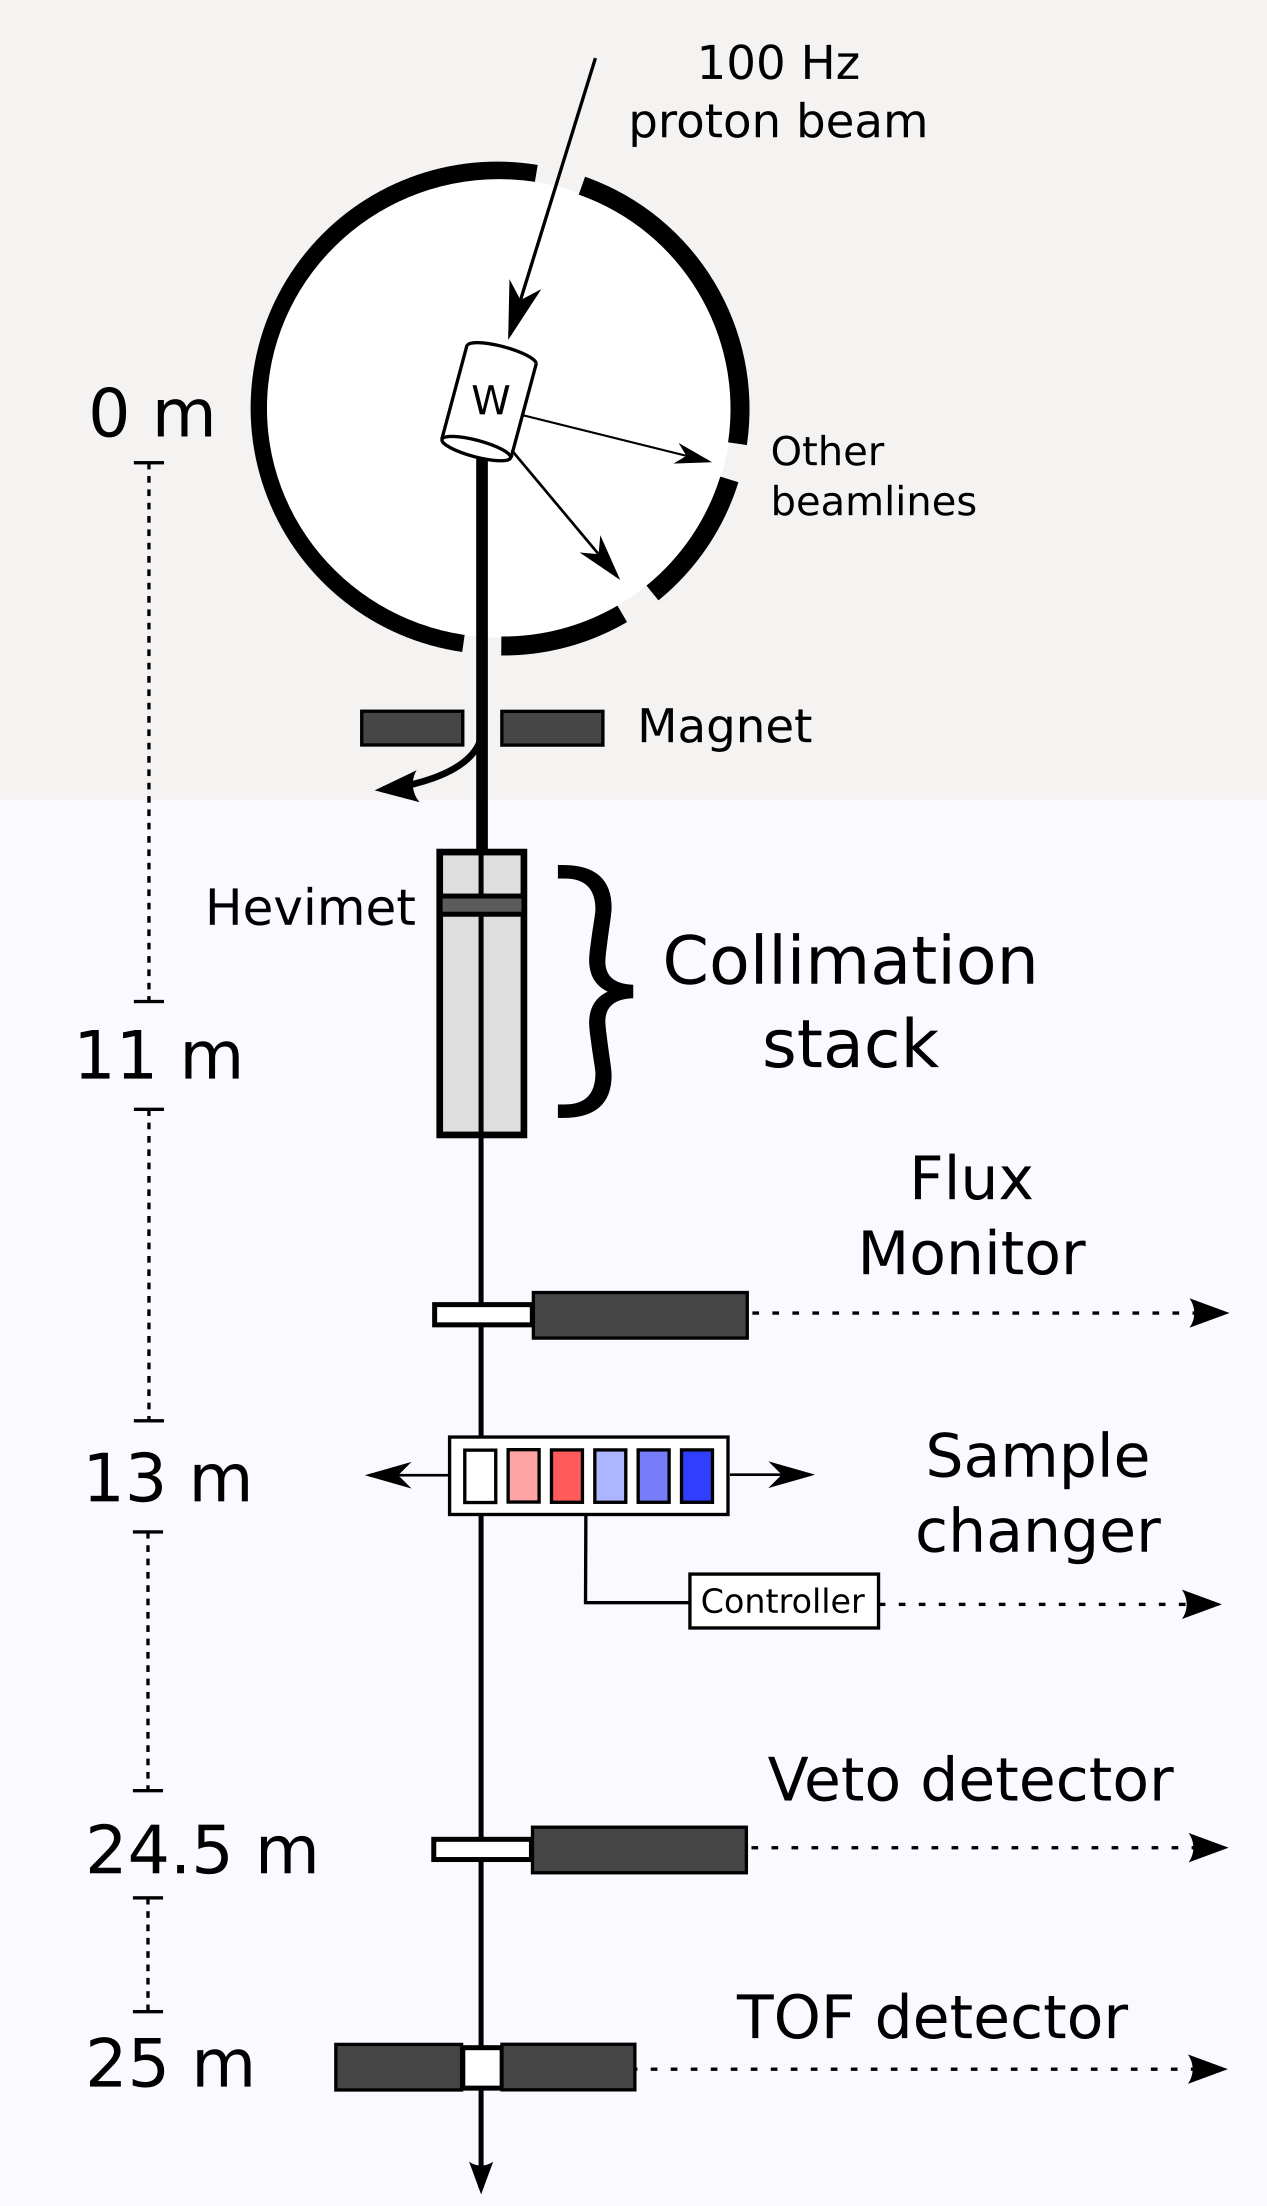
\includegraphics[scale=0.6]{figures/ExperimentalSetup.png}
    \caption{(Color online) Experimental configuration at WNR facility. After a
        permanent magnet sweeps charged particles from the beam, neutrons and
        $\gamma$ rays are collimated to a 0.200 inch beam en route to the
        detectors used in the experiment. Samples are cycled into and out of beam
        using a linear actuator with a period of 150 seconds. Times-of-flight (TOFs) are
    determined by the TOF detector and used to calculate neutron energy.}
    \label{ExperimentalApparatus}
\end{figure}

\begin{figure*}
    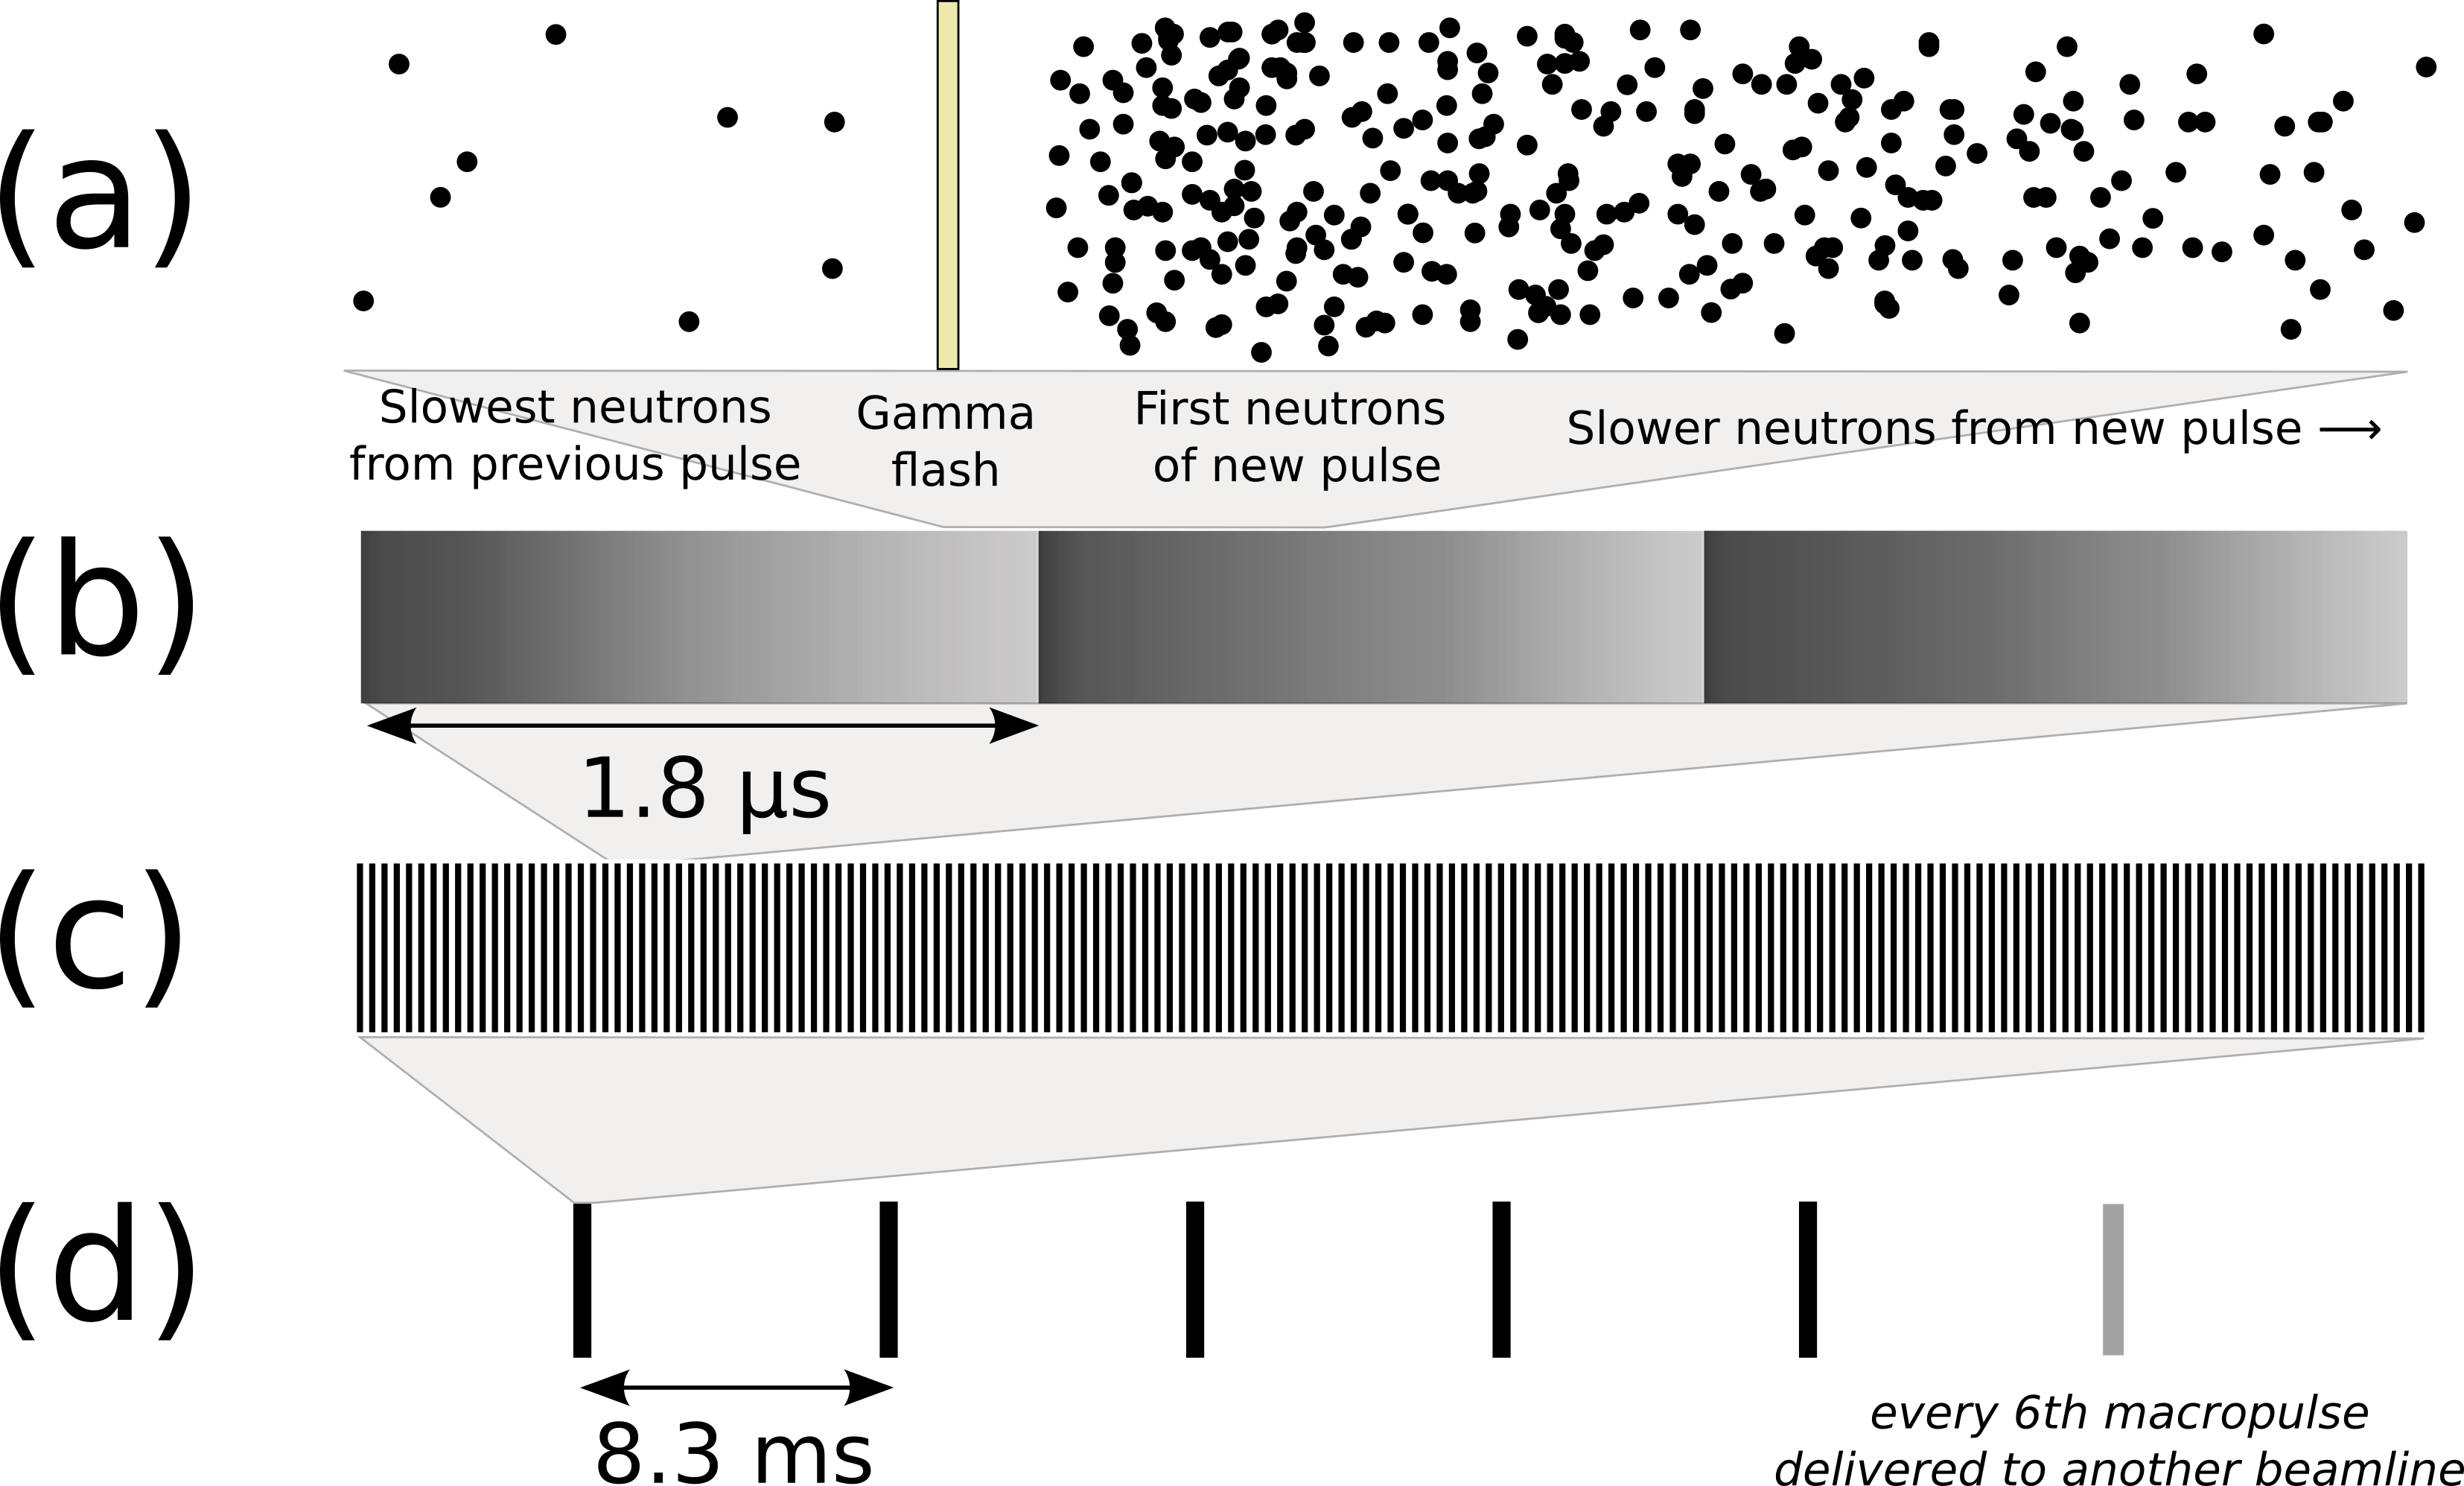
\includegraphics[scale=0.4]{figures/beamStructure.png}
    \caption{(Color online) Neutron beam structure at WNR facility. ``Macropulses" of protons (bottom row on figure) are delivered to Target 
        4, where they generate
        neutrons by spallation on a tungsten target. Each macropulse consists of
        $\approx$ 350 proton ``micropulses" (second from bottom row). Neutrons
        from each micropulse (second from top row) disperse in
        time as they travel along the flight path so that $\gamma$ rays and high-energy 
        neutrons catch up
to low-energy ones from the previous pulse.}
    \label{BeamStructure}
\end{figure*}

The particular neutron beam structure at WNR dictates the energy range
achievable for \tots measurements (see Fig. \ref{BeamStructure}).
Proton pulse trains, called ``macropulses", are delivered to the tungsten target at 120 Hz.
Each macropulse consists of ~350 individual proton pulses, called ``micropulses", spaced 1.8 
$\mu$s apart. Each micropulse consists of a single proton packet $<$1 ns wide when it 
arrives at the tungsten target that generates gamma rays and neutrons within a tight
temporal-spatial range. As neutrons from a single micropulse travel along the beam path, 
high energy neutrons sparate in time from lower-energy neutrons so that neutron
energy can be determined by standard TOF techniques (see \cite{Moore1980} for details).
Because the $\gamma$-rays and high-energy neutrons from later pulses can catch
up to slower neutrons from an earlier micropulse, the distance of the TOF
detector determines both the minimum neutron energy that can be unambiguously
detected and also the maximum instantaneous event rate, critical to correcting
for per-event deadtime.

A programmable sample changer with six positions
was used to cycle each sample into the beam at a regular interval of 150 seconds 
per sample. Once per macropulse, an analog signal from the sample changer was recorded to 
indicate the current position. Variations in beam flux 
between macropulses were monitored by the flux monitor detector. To account for
charged-particle production in the samples and in air along the flight path, a
veto paddle was installed immediately upstream of the TOF detector.

Custom digitizer software was used to run the 
digitizer in two complementary modes, referred to as "DPP mode" and "Waveform 
mode". In DPP mode, triggers were initiated by the digitizer's onboard
peak-sensing firmware. For each trigger, several quantities were recorded: the trigger 
timestamp, two charge integrals over the detected peak with different
integration ranges (32 ns for the short integral, 100 ns for the long integral),
and a 96-ns portion of the raw digitized waveform, referred to as a ``wavelet".
DPP mode was used for the vast majority of the 
experiment and accounts for $\approx$99\% of the total data volume. In waveform mode, 
the digitizer performs no peak-sensing and was externally triggered. Upon 
triggering, the trigger timestamp and a very long wavelet (60 $\mu$s) 
were recorded. While waveform mode data accounts for only $\approx$1\% of the total data, 
the instantaneous data rate is much higher than in DPP 
mode because hundreds of $\mu$s of consecutive waveform samples are 
stored. Roughly once every three seconds, the digitizer was switched to 
waveform mode for one macropulse, then immediately switched back to DPP mode.  

Except for the oxygen and rhodium samples, all samples were prepared as right
cylinders $\approx$8.25 mm in diameter and ranging from 10-27 mm in length (see
Table \ref{SampleTable} and Fig. \ref{SamplesImage}). A natural-abundance sample
was also prepared for each element under study as were two natural carbon
samples and a natural lead sample for benchmarking to literature. The samples
were inserted into styrofoam sleeves and seated in the cradles of the sample
changer. This design minimizes the amount of non-target mass proximate to the
neutron beam path.

\begin{table*}[ht]
    \caption{Sample Characteristics}
    \label{SampleTable}
    \begin{center}
        \begin{tabular}{ c c c c c c }
            \hline
            Isotope & Nat. Abund. & Sample Purity & Length [mm] & Diameter
            [mm] & Mass [g] \\
            \hline

            $^{nat}$C & - & - & 13.66$\pm$0.02 & 8.26$\pm$0.005 & 1.2363 \\
            $^{nat}$C & - & - & 27.29$\pm$0.02 & 8.26$\pm$0.005 & 2.4680 \\

            H$_{2}$$^{nat}$O & - & - & 20.0 & 10.0 & N/A \\
            D$_{2}$$^{nat}$O & - & - & 20.0 & 10.0 & N/A \\
            H$_{2}$$^{18}$O & 0.20\% & 99\% & 20.0 & 10.0 & N/A \\

            $^{58}$Ni & 68.077\% & 99.6\% & 7.97$\pm$0.03 & 8.18$\pm$0.02 &
            3.6438 \\
            $^{nat}$Ni & - & - & 8.00$\pm$0.03 & 8.20$\pm$0.02 &
            3.6898 \\
            $^{64}$Ni & 0.926\% & 92.2\% & 7.96$\pm$0.02 & 8.20$\pm$0.04 &
            3.9942 \\

            $^{103}$Rh & 100\% & 99.9\% & ?$\pm$? & ?$\pm$? & 2.8359 \\

            $^{112}$Sn & 0.97\% & 99.9\% & 13.65$\pm$0.03 & 8.245$\pm$0.005 &
            4.9720 \\
            $^{nat}$Sn & - & - & 13.68$\pm$0.03 & 8.245$\pm$0.005 &
            5.3263 \\
            $^{124}$Sn & 5.79\% & 99.9\% & 13.73$\pm$0.03 & 8.245$\pm$0.005 &
            5.5492 \\

            $^{nat}$Pb & - & - & 10.07$\pm$0.02 & 8.27$\pm$0.01 & 6.130 \\

            \hline
        \end{tabular}
    \end{center}
\end{table*}

The oxygen isotopes were prepared as water samples to increase the areal density
of atoms and for ease of handling. Each water sample was contained by a
cylindrical brass vessel with very thin (0.002 inch) brass endcaps, minimizing
beam attenuation in the vessel. Oxygen cross sections were calculated by
subtracting the well-known hydrogen cross section from the raw H$_{2}$O result
(we used H \tots data sets from Clement \cite{Clement1972} and Abfalterer 
\cite{Abfalterer2001}, which together cover the range $0.5 \leq E_n \leq 500$ MeV
and are in excellent agreement where their energy ranges overlap). Because of
the additional uncertainty inherent in this kind of subtractive \tots
determination, as an additional cross-check a D$_{2}^{nat}$O sample was also
prepared from which the literature \tots for D$_{2}$ could be subtracted to
recover the oxygen \tot. Due to its poor machining properties, the rhodium
sample was prepared by stacking a series of thin rhodium discs rather than by
producing a fused cylinder. These discs were contained by a cylindrical plastic
cas with open ends, similar to the styrofoam sleeves.

The sample configuration for each run varied, but generally all six positions on
the sample changer were used. For the solid targets, a typical configuration was
to place an empty styrofoam sample sleeve in the first sample-changer cradle as
the ``blank", the $^{nat}$C and $^{nat}$Pb samples in the second and third
cradles, and the samples of interest (e.g., $^{58}$Ni, $^{nat}$Ni, $^{64}$Ni) in
the fourth, fifth, and sixth cradles. For water samples, an empty brass vessel
was placed in the first cradle to serve as the blank.

\begin{figure}
    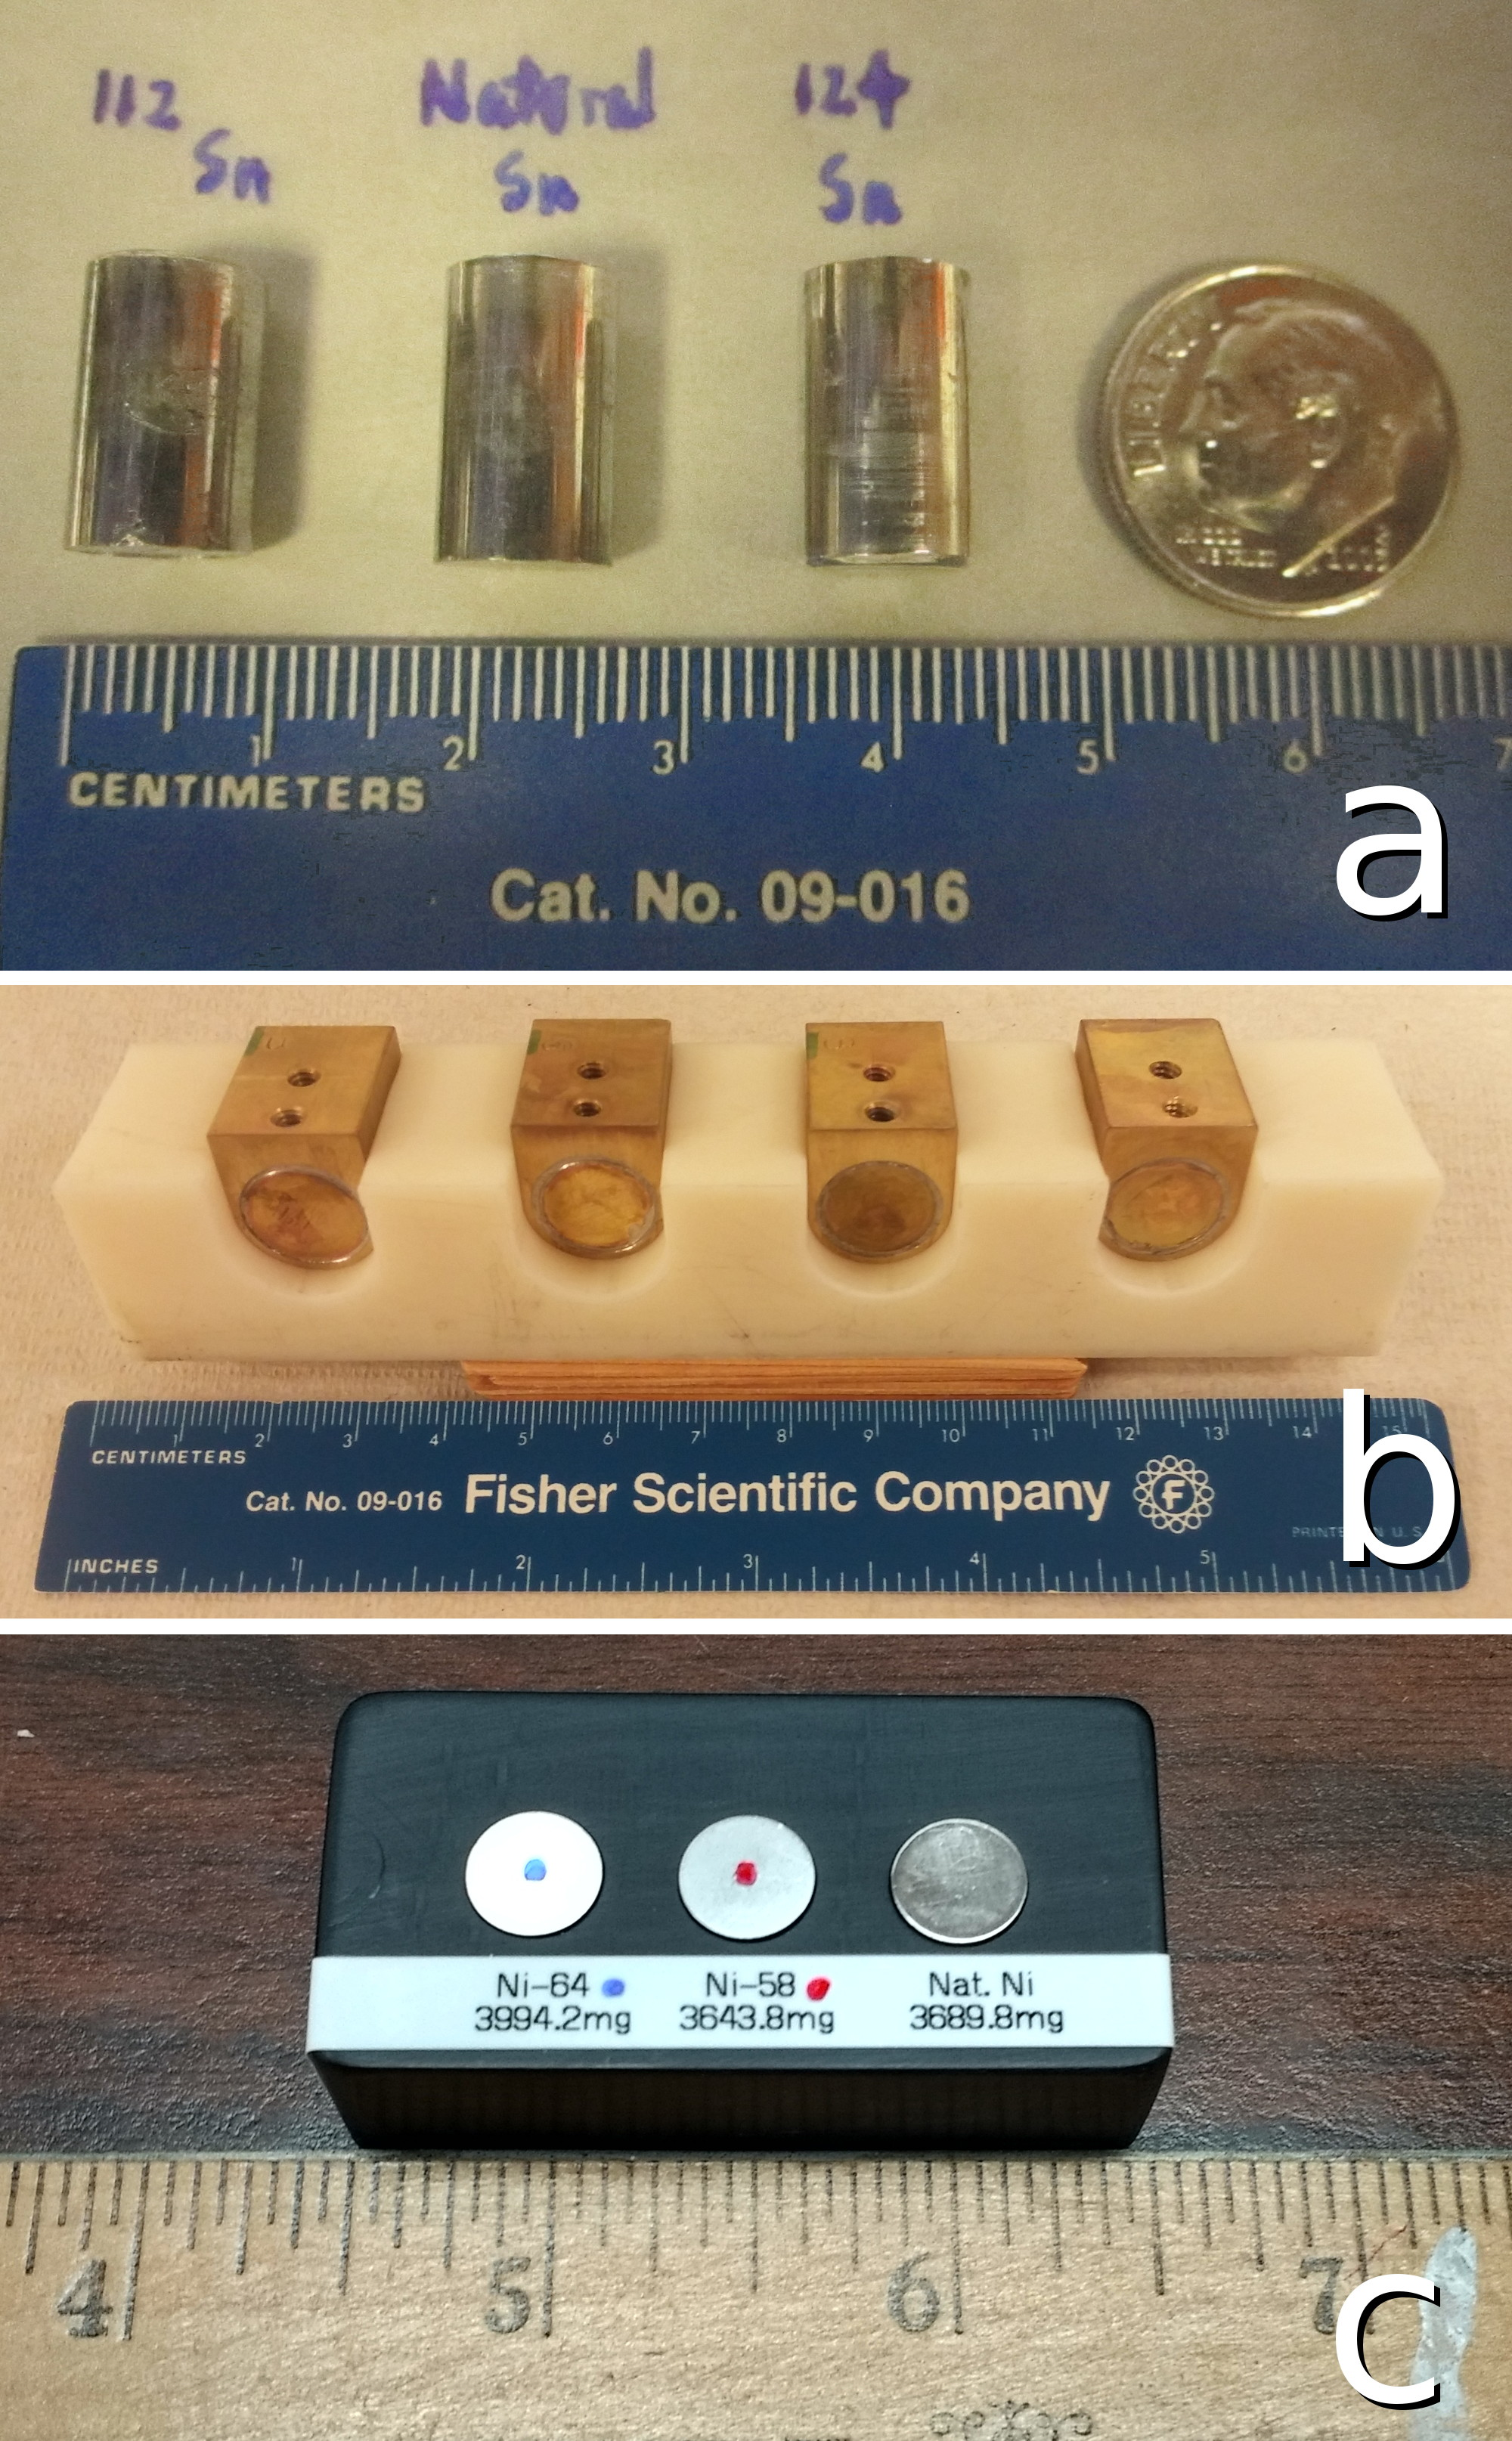
\includegraphics[scale=0.23]{figures/AllIsotopicSamples.jpg}
    \caption{(Color online) Section (a): the ${^{112,nat,124}}$Sn samples. Section (b): the 
        vessels used to hold water samples for the ${^{nat, 18}}$O \tots measurement. 
        Section (c): ${^{58,nat,64}}$Ni samples, shown end-on.}
    \label{SamplesImage}
\end{figure}

\section{Analysis}

The fundamental quantity of interest, \tot, is related to the flux
loss through a sample by:

\begin{equation}
I_{t} = I_{0}e^{-{\ell\rho\sigma_{tot}}}
\end{equation}

or, equivalently,

\begin{equation}
    \tot = -\frac{1}{\ell\rho}ln\left(\frac{I_{t}}{I_{0}}\right)
\end{equation}

where $I_{0}$ is the neutron flux entering the sample, $I_{t}$ is the neutron
flux transmitted through the sample without interaction, $\rho$ is the number
density of nuclei in the sample, and $\ell$ is the sample length. Thus for thin
or low-density samples, flux attentuation through the sample will be very small
($\approx$[insert attenuation \% here] for our Ni samples) and a large number
of counts will be required to determine the cross section with high
precision.

To calculate cross sections from raw event data, a series of corrections are
required. First, all macropulse start times were identified and each event was
assigned to the correct macropulse. Time offsets (accounting for cable and
electronics delay) were applied, roughly synchronizing all detectors with
facility-provided $T_{0}$ pulses (capacitive pick-off signals that
indicate the arrival of proton pulses on the tungsten target and thus serve as
the TOF start time for each micropulse). The digitized waveform for each event was passed through an
offline software CFD logic, improving the timing resolution for each event to
below 1 ns [insert FWHM from left/right detectors here].

To improve the macropulse start time resolution and test the stability of the
micropulse period during a macropulse, all $\gamma$ rays for a given macropulse
were identified and their average TOF calculated. The difference between this
time and the expected TOF (given the TOF detector distance and speed of light)
was applied to all events in that macropulse (see Fig.
\ref{TimingCorrectionStudy}). The final time resolution (i.e., FWHM of the
$\gamma$-ray peak in the TOF spectra) ranged from 0.60-0.85 ns over the series of
\tots measurements and is comparable to the resolution from our Ca experiment
from 2008 \cite{Shane2010}. For a 100-MeV neutron, an uncertainty of 0.80 ns in
the macropulse start time translates to an energy resolution of $\approx$880
keV. For neutrons below $\approx$10 MeV, the traversal time through
the 1-inch thickness of the TOF detector starts to contribute significantly
to timing uncertainty. However, because the TOF of these neutrons is already at
least several hundred ns, the energy resolution ($\frac{\Delta E}{E}$) is
superior at low energies (for a 5 MeV neutron with a 0.82 ns detector-traversal time and
0.80 ns inherent timing uncertainty, $\Delta E$ is 13 keV). These energy uncertainties
have been properly propagated through analysis and are shown as error bars in our \tots 
results below.

Determination of the TOF distance was done by comparing our measured \totEs data
for $^{nat}$C with that from literature from 3-15 MeV, the results of which are
shown in Fig. \ref{DistanceStudy}. The distance was determined as 2709$\pm$1 cm
for the Ni and Rh measurement and 2554$\pm$1 cm for the Sn and O measurement.

Because events are not processed instantaneously, there is a brief period,
referred to as the "analytic deadtime", after each event trigger during which
the digitizer is busy processing that trigger. Any newly-arriving events in this
period will be ignored, privileging events arriving earlier and thus distorting
the cross sections.

To remedy this, a deadtime correction for
each target must be calculated and applied according to standard techniques
\cite{Moore1980}. Assuming negligible variation in beam flux between micropulses
(an assumption investigated), the deadtime correction formulae described by
Moore
fraction of time $F[i]$ that the digitizer is dead for a given time bin $i$ can
be calculated:

\begin{equation}
    F_{i} = \sum^{N-1}_{j=0} R_{i-j\text{ (mod N)}}\times P_{j}
\end{equation}
where $N$ is the number of time bins in the micropulse, $R_{x}$ is the number of
events per micropulse in bin $x$, and $P_{x}$ is the probability that the
digitizer is still busy from a trigger $x$ bins ago. To model $P_{j}$, we
employed a logistic function and fitted it to the observed spectrum for time
differences between consecutive events (see Fig.
\ref{TimeDifferenceBetweenEvents}). For a given bin $i$, the fraction of time that the 
digitizer is dead, $F_{i}$, is in essence a discrete convolution of the
\textit{measured} TOF spectrum with $P_{j}$. Note that except for the first and
last micropulses in a macropulse, micropulses are
consecutive with no delay between them and thus deadtime effects can
``wrap around" from the end of one micropulse to the next. For these wrap-around
contributions (that is, $j>i$), the (mod N) term ensures that the bin referred
to by $i-j$ is non-negative and has physical meaning as a time bin from the previous 
micropulse.

\begin{figure}
    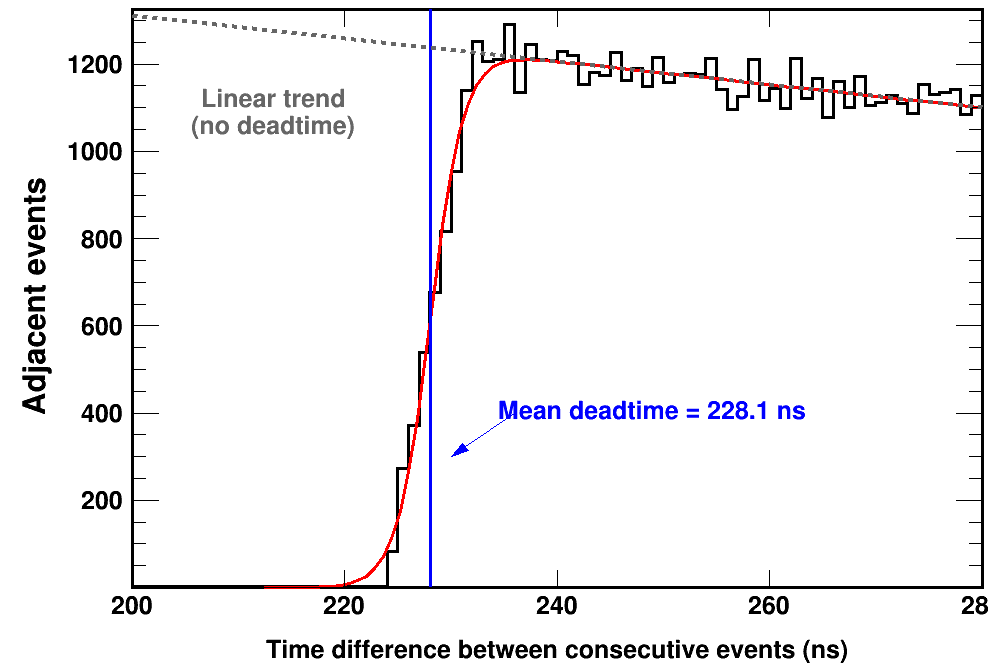
\includegraphics[scale=0.24]{figures/TimeDifferenceBetweenEvents.png}
    \caption{(Color online) The time difference between adjacent TOF-detector
    events for a single run is plotted (black histogram). Below a certain
minimum time difference (the ``deadtime"), no events are recorded. A logistic
fit (red) models the detector's deadtime response and is used to generate a
deadtime correction. The underlying linearly-decreasing count rate (gray dashed
line) in incorporated into the logistic model. From the fit, a mean deadtime of
228.1 ns was extracted for the Sn and O run configurations (a similar
procedure was used to recover a deadtime of [insert deadtime] for the Ni and Rh
run configurations).}
    \label{TimeDifferenceBetweenEvents}
\end{figure}

\begin{figure*}
    \includegraphics[scale=0.3]{figures/distanceStudy.png}
    \caption{(Color online) Results of a study to determine the distance between
    the neutron source and the TOF detector for the Ni/Rh running configuration
are shown. First, a plausible range of flight path distances was selected based
on rough estimation during the experiment (26.97-27.21 m). For each of several
distances in this range, the \totEs for natural carbon was calculated in the
resonance region (3-15 MeV). then the RMS difference between our cross section
(calculated using that distance) and literature data from Abfalterer
\cite{Abfalterer2000, Abfalterer2001} was calculated (shown as black points in
the figure). A quartic fit to these RMS data is shown in red. By minimizing the
RMS difference, we calculate a flight path distance of 2709$\pm$1 cm.}
    \label{DistanceStudy}
\end{figure*}

Typical values for $F_{i}$ in our experiment are shown in Fig.
\ref{ExampleDeadtimeSpectrum}. Because trigger processing is done quickly in
firmware onboard the digitizer, the per-event deadtimes affecting our
measurement ranged from 150-230 ns, much smaller than the several-$\mu$s
deadtime-equivalents in previous analog experiments \cite{Finlay1993,
Abfalterer2001}.

One the fraction dead was identified for each time bin, the number of events
\textit{measured} in that bin, $N_{m}[i]$, was corrected to the \textit{true}
number of events $N_{t}[i]$ that would have been detected in that bin in the absence of
analytic deadtime effects:

\begin{equation}
    N_{t}[i] = -ln\left(\frac{1-\frac{N_m[i]}{M}}{(1-F_{i})\times M}\right)
\end{equation}

where M is the total number of micropulse periods. The difference between
uncorrected and corrected TOF spectra is shown in Fig.
\ref{CorrectionEffectOnTOF}. At large TOFs (low energies) the correction is as low as a
few percent, but at small TOFs (high energies) when the digitizer is still dead
from the gamma flash and high-energy neutrons, the correction to TOF is significant
($approx$20\% for our Ni/Rh runs, and $\approx$40\% for our Sn/O runs). However, these corrections are far lower than the typical
deadtime correction required using the analog approach \cite{Finlay1993,
Abfalterer2001} that were as high as 500\%. The propagation of our correction to the final 
cross section results is shown in Fig. \ref{DeadtimeEffectOnCS}.

\begin{figure*}
    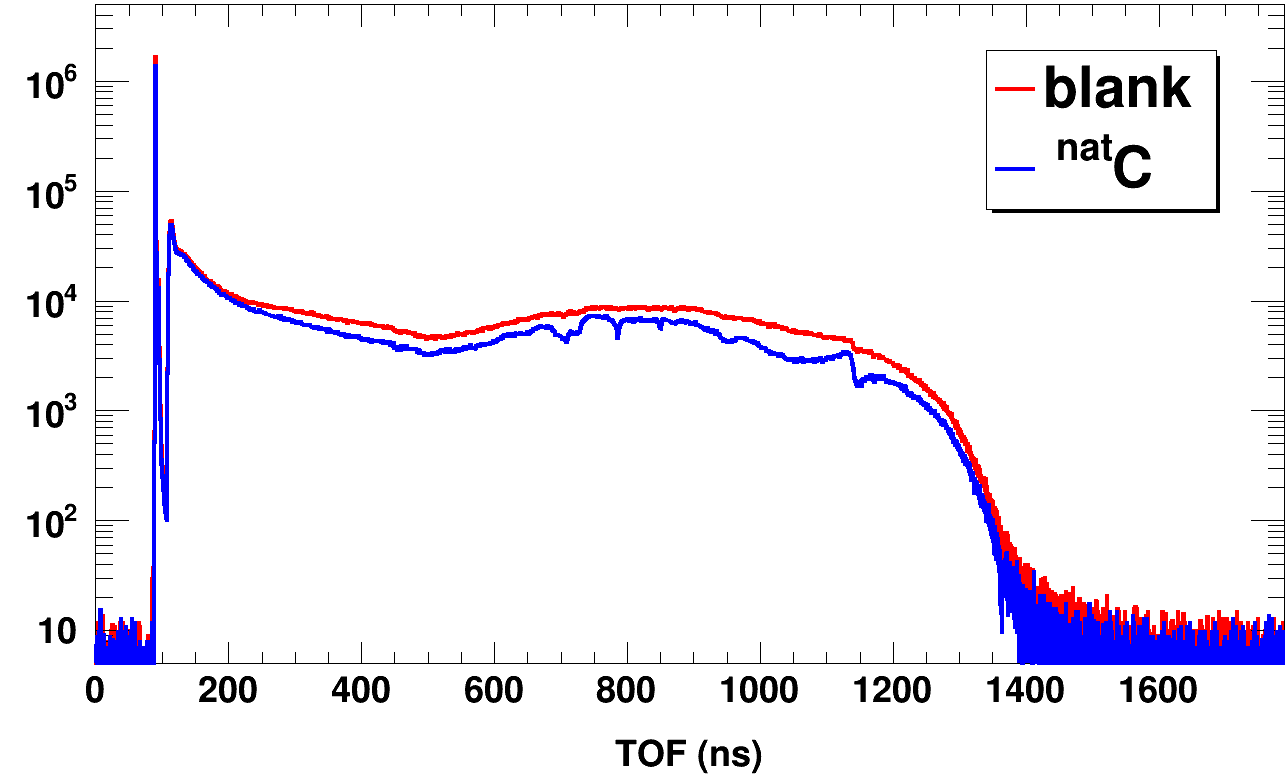
\includegraphics[scale=0.3]{figures/exampleTOFSpectrum.png}
    \caption{(Color online) The TOF spectrum is shown for the blank sample (in
        red) and for the $^{nat}$C sample (in blue) from the Ni/Rh experiment.
        The $\gamma$-ray peak is visible as a sharp spike at 90 ns, followed by
        the highest-energy neutrons at $\approx$130ns. Events caused by accelerator 
        "dark current" are visible as 
    }
    \label{ExampleTOFSpectrum}
\end{figure*}

\begin{figure*}
    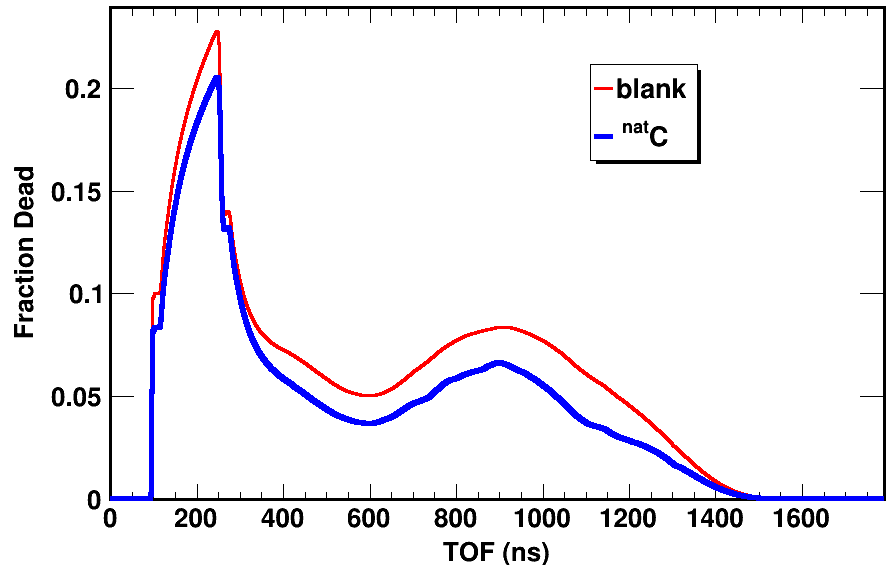
\includegraphics[scale=0.3]{figures/exampleDeadtimeSpectrum.png}
    \caption{(Color online) Using TOF data from a typical run, the probability that a given 
        TOF bin is ``dead" is shown for the blank sample (in red) and the $^{nat}$C sample 
        (in blue). Note the sharp rise at 90 ns corresponding to the
        $\gamma$-ray flash, the gradual increase from 90-245 ns corresponding to
        the arrival of high energy neutrons, and the sharp fall at 245 ns
        corresponding to the elapse of the $\gamma$ ray deadtime ``shadow". Only high-
        energy neutrons have a probability-dead $>$10\% (cf. the 50-80\%
        probability-dead of \cite{Finlay1993, Abfalterer2001}).
    }
    \label{ExampleDeadtimeSpectrum}
\end{figure*}

\begin{figure*}
    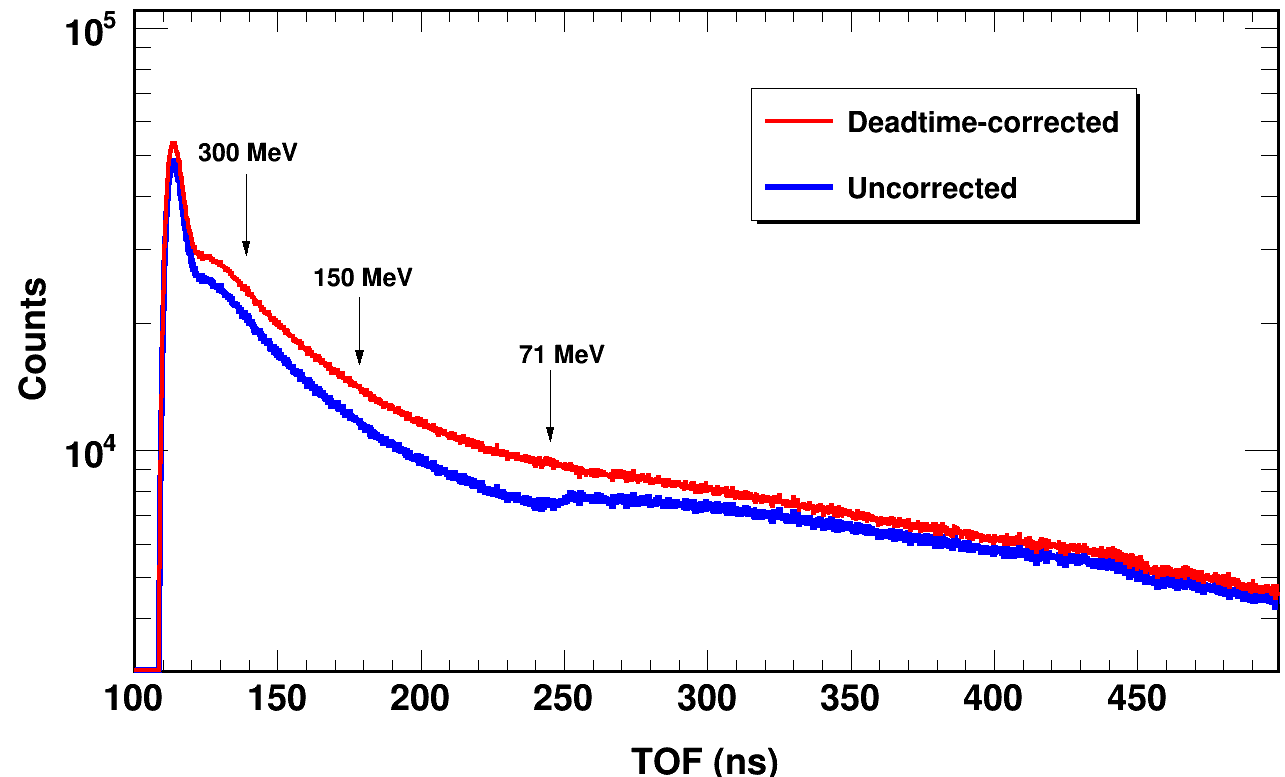
\includegraphics[scale=0.3]{figures/CorrectionEffectOnTOF.png}
    \caption{(Color online) A typical TOF spectrum from the Ni/Rh
        run configuration is shown, before (in blue) and after (in red) analytic
        deadtime correction. Relevant neutron energies are indicated above the spectra.
        For this digitizer configuration, the mean deadtime was 155 ns (see Fig.
        \ref{TimeDifferenceBetweenEvents} for details on mean deadtime determination).
        Note that at 245 ns, there is an
        obvious defect in the uncorrected spectrum is repaired in the corrected
        spectrum. The defect
        corresponds to the elapse of the deadtime ``shadow" from the $\gamma$
        ray flash that came 155 ns earlier at $\approx$90 ns (not pictured).
    }
    \label{CorrectionEffectOnTOF}
\end{figure*}

In addition to per-event deadtime, a "readout deadtime", from digitizer readout 
to the data acquisition computer (DAQ), must be accounted for. Each pair of
digitizer channels shares a common buffer for storing events; upon reaching a
user-defined threshold, buffer contents are read out to the DAQ as packets.
During readout, the digitizer is ...something.
This is likely the largest source of systematic error in our measurement.

After applying deadtime and gamma correction, vetoed events are removed and
integrated charge gates are applied to remaining TOF events.
Surviving events are populated into energy spectra. The cross section was
calculated, bin-wise, as follows:

$$
\tot = -\frac{1}{\ell\rho}
ln \left(\frac{I_{0}}{I_{s}}\times\frac{F_{s}}{F_{0}}\right)
$$

where $\frac{I_{0}}{I_{s}}$ is the ratio of counts in energy spectra between 
the blank and sample, $\frac{F_{s}}{F_{0}}$ is the ratio of beam flux
between the sample and blank, $\ell$ is the length of the sample, and $\rho$ is the
number density of atoms in the sample.

[More here with a comparison between Bec's and Abfalterer/Finlay's approach to
the same issues].

During analysis, it was noted that occasionally (\~1 in 400 macropulses), one or two 
adjacent macropulses would have an abnormally small number of flux monitor events or 
TOF events. The frequency of these "data dropouts" was similar to the rate of
switching between DPP and waveform modes and we suspect it is related to edge
case behavior right before or after a mode switch. To mitigate this issue,
any macropulse that had less than 50\% of the average event rate in either the
flux monitor or TOF detector channel was ignored during cross section calculation.

After the above corrections, the charged-particle veto was applied. 

[more description here about gamma ray timing precision and a comparison to
that from Bec's experiment].

[describe veto procedure, charge gating procedure, and conversion of TOF to
energy bins]

\section{Error Analysis}

[describe error propagation...? Or this more appropriate for analysis section?]

\section{Experimental Results}

[all cross section plot results]

\section{Discussion}

[Discussion]

\section{DOM Analysis}

[Preliminary DOM Analysis for oxygen]

\section{Conclusion}

[Conclusion]

\section{Acknowledgements}

\begin{figure*}
    \includegraphics[scale=0.35]{figures/FourPanelO.png}
    \caption{(Color online) Neutron total cross sections for $^{16,18}$O.
     Panel one shows our measurement (in red) and literature data from
     Abfalterer (in
     black), where the $^{18}$O values have been shifted up by 1 barn for
     readability. Panel two shows the relative difference between our 
     measurement and the literature data from the first panel. Panels three and
     four show the corresponding absolute and relative cross sections after a
     Pb-C correction, derived from literature data and our Sn dataset,
     are applied.
    }
\end{figure*}

\begin{figure*}
    \includegraphics[scale=0.35]{figures/FourPanelNi.png}
    \caption{(Color online) Neutron total cross sections for $^{58,64}$Ni.
     Panel one shows our measurement (in red) and literature data from
     Abfalterer (in % black).
     Panel two shows the relative difference between our 
     measurement and the literature data from the first panel. Panels three and
     four show the corresponding absolute and relative cross sections after a
     Pb-C correction, derived from literature data and detailed in the text,
     are applied.
    }
\end{figure*}

\begin{figure*}
    \includegraphics[scale=0.35]{figures/FourPanelSn.png}
    \caption{(Color online) Neutron total cross sections for $^{112,124}$Sn.
     Panel one shows our measurement (in red) and literature data from
     Finlay (in % black).
     Panel two shows the relative difference between our 
     measurement and the literature data from the first panel. Panels three and
     four show the corresponding absolute and relative cross sections after a
     Pb-C correction, derived from literature data and detailed in the text,
     are applied.
    }
\end{figure*}

\begin{figure*}
    \includegraphics[scale=0.35]{figures/FourPanelNiIsotopes.png}
    \caption{(Color online) Neutron total cross sections for $^{58,64}$Ni.
     Panel one shows our measurement (in red) and literature data from
     Abfalterer (in % black).
     Panel two shows the relative difference between our 
     measurement and the literature data from the first panel. Panels three and
     four show the corresponding absolute and relative cross sections after a
     Pb-C correction, derived from literature data and detailed in the text,
     are applied.
    }
\end{figure*}

\begin{figure*}
    \includegraphics[scale=0.35]{figures/FourPanelSnIsotopes.png}
    \caption{(Color online) Neutron total cross sections for $^{112,124}$Sn.
     Panel one shows our measurement (in red) and literature data from
     Finlay (in % black).
     Panel two shows the relative difference between our 
     measurement and the literature data from the first panel. Panels three and
     four show the corresponding absolute and relative cross sections after a
     Pb-C correction, derived from literature data and detailed in the text,
     are applied.
    }
\end{figure*}


\bibliography{references}
\begin{thebibliography}{32} \expandafter\ifx\csname
        natexlab\endcsname\relax\def\natexlab#1{#1}\fi \expandafter\ifx\csname
        bibnamefont\endcsname\relax \def\bibnamefont#1{#1}\fi
        \expandafter\ifx\csname bibfnamefont\endcsname\relax
        \def\bibfnamefont#1{#1}\fi \expandafter\ifx\csname
        citenamefont\endcsname\relax \def\citenamefont#1{#1}\fi
        \expandafter\ifx\csname url\endcsname\relax \def\url#1{\texttt{#1}}\fi
        \expandafter\ifx\csname urlprefix\endcsname\relax\def\urlprefix{URL
        }\fi \providecommand{\bibinfo}[2]{#2}
        \providecommand{\eprint}[2][]{\url{#2}}

\end{thebibliography}

\end{document}
